\subsection{Externe Abhängigkeiten}
\label{sec:model_external_dependencies}

Unter \textit{External Dependencies} sind die Aspekte zusammengefasst, die eine Auswirkung auf die Erklärungen in einem System haben. Aus den hier vorgestellten Aspekten können im Anschluss Anforderungen und Einflusshypothesen für Erklärungen aufgestellt werden. Daraus kann dann auch abgeleitet werden, welche Funktionen des Systems einer Erklärung bedürfen \cite{kohl_explainability_2019}. Im Folgenden werden die beiden zusammenhängenden Unteraspekte \textit{Context} des Systems und \textit{Objectives} erläutert.

\subsubsection{Context}

Der \textit{Context} einer Erklärung beschreibt die äußeren Einflüsse, die unmittelbar auf das erklärbare System wirken und aus denen somit Anforderungen an die Eigenschaften von Erklärungen abgeleitet werden können. Einen Überblick über den \textit{Context} bietet \autoref{fig:model_context_overview}.

\begin{figure}[htb!]
    \begin{center}
        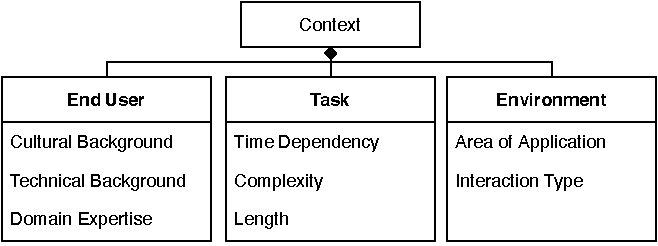
\includegraphics{contents/05_model_description/res/model_context_overview.pdf}
    \end{center}
    \caption{Übersicht über den \textit{Context} eines erklärbaren Systems}
    \label{fig:model_context_overview}
\end{figure}

Dies beinhaltet die Aktivität, die der Endbenutzer in einer bestimmten Umgebung durchführt. Aus den Eigenschaften der drei Aspekte (Aktivität, Endbenutzer und Umgebung) leiten sich dabei direkte Einflüsse auf den Bedarf, den Inhalt und die Darstellung einer Erklärung ab. \autoref{tab:impact_of_context_on_explanation} stellt die verwendeten Synonyme für die verschiedenen Facetten des \textit{Context} eines Systems dar.
% Insbesondere der Begriff Stakeholder wurde in der Literatur verschieden eingesetzt. \citeauthor{cirqueira_scenario-based_2020} nutzen den Begriff für den Nutzer einer Software \cite{cirqueira_scenario-based_2020} während \citeauthor{nunes_systematic_2017} diesen als Oberbegriff für Personengruppen, die ein Interesse an einem System haben, verwenden, den Nutzer allerdings ausschließen \cite{nunes_systematic_2017}. Diese Arbeit verwendet den Begriff, um alle Personengruppen mit Interesse am System inklusive aller Nutzer zu beschreiben (\cite[vgl.][]{schneider2012abenteuer,chazette_knowledge_nodate}).
Folgend werden nun die drei Aspekte sowie typische Ausprägungen oder Charakteristiken näher erläutert.

\begin{table}[bht!]
    \begin{tabular}{p{.2\textwidth}p{.4\textwidth}p{.31\textwidth}}
        \hline
        Aspekt & Synonyme & Quellen \\
        \toprule
        End User        &  (Targt / End)  User & \cite{chazette2020explainability} \cite{kaptein_personalised_2017} \cite{sokol_one_2020} \cite{wiegand_id_2020} \\
                        & Stakeholder & \cite{chazette_knowledge_nodate} \\
                        & Consumer & \cite{ehsan_human-centered_2020} \\
                        & Explainee & \cite{chazette_knowledge_nodate} \cite{kohl_explainability_2019} \\
                        & Explanation Audience & \cite{sokol_explainability_2020} \\
        \tablerowspacing
        Task            & Task & \cite{chazette_knowledge_nodate} \cite{sokol_explainability_2020} \cite{gunning2019darpa} \\
                        & Activity & \cite{wohlin2012experimentation} \\
        \tablerowspacing
        Environment     & Environment & \cite{chazette_knowledge_nodate} \cite{wiegand_id_2020} \cite{wiegand2019drive} \\
                        & Application Area & \cite{sokol_explainability_2020} \cite{wiegand2019drive} \cite{wiegand_id_2020} \\
        \toprule
    \end{tabular}
    \caption{Relevante Aspekte des \textit{Context} eines erklärbaren Systems zur Integration von Erklärungen}
    \label{tab:impact_of_context_on_explanation}
\end{table}

\paragraph{End User} Der \textit{End User} ist diejenige Person, die mit dem System interagiert und auf welchen somit die Erklärungen zugeschnitten sein müssen. Dieser entspricht in den Definitionen von Erklärbarkeit von \citeauthor{chazette_knowledge_nodate} sowie von \citeauthor{kohl_explainability_2019} dem \textit{Explainee} \cite{chazette_knowledge_nodate, kohl_explainability_2019}. Allerdings muss der \textit{Explainee} nicht zwangsweise \textit{End User} des Systems sein, sondern einer anderen Stakeholdergruppe angehören.

Generell kann ein System verschiedene Nutzer(-typen) haben, die sich in ihrem Bedarf für Erklärungen unterscheiden. Im Folgenden werden die am häufigsten erwähnten Eigenschaften vorgestellt (unter anderem in \cite{chazette_knowledge_nodate,tintarev_designing_nodate,yamada_evaluating_2016}).

Sowohl beim generellen technischen Verständnis (\textit{Technical Background}) als auch beim Domänen-Wissen (\textit{Domain Expertise}) \cite{yamada_evaluating_2016} können \textit{End User} verschieden viel Hintergrundwissen vorweisen. Somit können sich in einem System mit unterschiedlichen Eigenschaften der  Nutzer auch verschiedene Anforderungen an Erklärungen ergeben.

Der \textit{Cultural Background} fasst darüber hinaus die kulturellen Hintergründe von \textit{End Usern} zusammen, die sich zum Beispiel auf die Verwendung von Metaphern in Software bzw. Erklärungen auswirken können \cite{salgado_cultural_2015}.

\paragraph{Task} Der \textit{Task} definiert die Aufgabe(n), welche durch die \textit{End User} mithilfe des Systems durchgeführt werden sollen. Auch hier spielen verschiedene Eigenschaften eine Rolle. Genannt werden in der Literatur beispielsweise die Zeitabhängigkeit (\textit{Time Dependency}), die Komplexität (\textit{Complexity}) und die Dauer der Aufgabe (\textit{Length}). Die drei genannten Ausprägungen werden als wichtige Betrachtungsgegenstände für die Eigenschaften von Erklärungen beschrieben. Daraus resultierend sind auch diese Aspekte für die Anforderungserhebung im Kontext der Erklärbarkeit relevant \cite{sokol_explainability_2020}.

\paragraph{Environment} Sehr eng mit der zu erledigenden Aufgabe hängt auch dessen Umgebung zusammen. Das \textit{Environment} ist durch die äußeren Umstände des Systems definiert. Dies beinhaltet den generellen Anwendungsbereich des Systems (\textit{Area of Application}), welcher unter anderem die Kri­ti­ka­li­tät eines Systems definiert. Aber auch die Art der Interaktion zwischen \textit{End User} und System fällt in diesen Bereich (\textit{Interaction Type}) und hat eine Auswirkung auf die Anforderungen an Erklärungen \cite{wiegand_id_2020}. 

\bigskip

Als Zwischenergebnis für \textbf{RQ1} kann festgehalten werden, dass der \textit{Context} eines Systems eine der zu betrachtenden Rahmenbedingungen mit einem Einfluss auf die Anforderungen an Erklärungen ist.

\subsubsection{Zielsetzung}
\label{subsec:model_objective}

Als zweiter Aspekt neben dem \textit{Context} werden in der Literatur die \textit{Objectives} für die Integration von Erklärungen mit einem Einfluss auf die Anforderungen an Erklärungen genannt \cite{rosenfeld_explainability_2019, nunes_systematic_2017}. 

\begin{table}[b!]
    \begin{center}
        \begin{tabular}{p{.2\textwidth}p{.4\textwidth}p{.31\textwidth}}
            \hline
            Qualitätsaspekt    & Beschreibung & Quellen \\
            \toprule
            Trust                       & Das Vertrauen des Nutzers in das System erhöhen \cite[vgl.][]{balog_measuring_2020}
                                        & \cite{nunes_systematic_2017} \cite{chazette_knowledge_nodate} \cite{tintarev_designing_nodate} \cite{balog_measuring_2020} \cite{eiband_impact_2019} \cite{tintarev2015explaining} \cite{hernandez-bocanegra_effects_2020} \cite{stange_effects_2021} \cite{weitz_you_2019} \cite{yamada_evaluating_2016} \cite{haspiel_explanations_2018} \cite{martin_developing_2019} \cite{martin_evaluating_2021} \cite{tsai_effects_2020}  \cite{sokol_one_2020}  \cite{wang_is_2018} \cite{koo_understanding_2016} \cite{wiegand2019drive} \cite{gunning2019darpa} \cite{lim_2009_assessing} \cite{tintarev2007survey} \cite{kunkel_let_2019} \\
            \tablerowspacing
            Satisfaction                & Die Benutzerfreundlichkeit und generelle Zufriedenheit von Nutzern mit dem
                                            System erhöhen. \cite[vgl.][]{balog_measuring_2020}
                                        & \cite{nunes_systematic_2017} \cite{chazette_knowledge_nodate} \cite{tintarev_designing_nodate} \cite{balog_measuring_2020} \cite{tsai_evaluating_2019} \cite{tintarev2015explaining} \cite{riveiro_thats_2021} \cite{martin_developing_2019} \cite{martin_evaluating_2021} \cite{tsai_effects_2020} \cite{ehsan_human-centered_2020} \cite{sovrano_modelling_2020} \cite{koo_understanding_2016} \cite{ribera2019can} \cite{gunning2019darpa} \cite{lim_2009_assessing}  \cite{tintarev2007survey} \cite{sato_context_nodate} \\
            \tablerowspacing
            Transparency                & Erklären, wie das System funktioniert. \cite[vgl.][]{balog_measuring_2020}
                                        & \cite{nunes_systematic_2017} \cite{chazette_knowledge_nodate} \cite{tintarev_designing_nodate} \cite{chazette_end-users_nodate} \cite{balog_measuring_2020} \cite{chazette2020explainability} \cite{tintarev2015explaining} \cite{hernandez-bocanegra_effects_2020} \cite{tsai_effects_2020} \cite{rjoob_towards_2021}  \cite{sokol_one_2020} \cite{wang_is_2018} \cite{koo_understanding_2016} \cite{tintarev2007survey}
                                        \cite{martin_evaluating_2021} \cite{ehsan_human-centered_2020}
                                        \cite{cheng2019explaining} \\
            \tablerowspacing
            Scrutability                & Nutzern die Möglichkeit geben, dem System einen Fehler mitzuteilen \cite[vgl.][]{balog_measuring_2020}
                                        & \cite{nunes_systematic_2017} \cite{chazette_knowledge_nodate} \cite{tintarev_designing_nodate} \cite{balog_measuring_2020} \cite{tintarev2015explaining} \cite{martin_developing_2019} \cite{gunning2019darpa}  \cite{tintarev2007survey} \cite{martin_evaluating_2021} \\
            \tablerowspacing
            Effectiveness               & Die Qualität der Aufgaben von Nutzern erhöhen \cite[vgl.][]{balog_measuring_2020}
                                        & \cite{nunes_systematic_2017} \cite{chazette_knowledge_nodate} \cite{tintarev_designing_nodate} \cite{balog_measuring_2020} \cite{tintarev2015explaining} \cite{zolotas_towards_2019} \cite{hernandez-bocanegra_effects_2020} \cite{martin_evaluating_2021} \cite{rjoob_towards_2021} \cite{tintarev2007survey} \\
            \tablerowspacing
            Efficiency                  & Nutzern helfen ihre Aufagaben schneller zu erledigen \cite[vgl.][]{balog_measuring_2020} 
                                        & \cite{nunes_systematic_2017} \cite{chazette_knowledge_nodate} \cite{tintarev_designing_nodate} \cite{balog_measuring_2020} \cite{tsai_evaluating_2019} \cite{tintarev2015explaining} \cite{hernandez-bocanegra_effects_2020} \cite{tintarev2007survey}\\
            \tablerowspacing
            Persuasiveness              & Die Akzeptanz der Entscheidungen des Systems durch die Nutzer erhöhen \cite[vgl.][]{balog_measuring_2020}
                                        & \cite{nunes_systematic_2017} \cite{tintarev_designing_nodate} \cite{balog_measuring_2020} \cite{sato_context_nodate} \cite{abdulrahman_belief-based_2019} \cite{tintarev2015explaining} \cite{sato_action-triggering_2019} \cite{tintarev2007survey} \\
            \toprule
        \end{tabular}
    \end{center}
    \caption{Untersuchte Qualitätsaspekte in der Literatur für die Qualitätsbestimmung von Erklärungen mit Definition}
    \label{tab:quality_aspects_of_explanation}
\end{table}

\citeauthor{chazette_knowledge_nodate} haben in ihrem Modell für Erklärbarkeit die Qualitätsaspekte zusammengefasst, die mit Erklärbarkeit in einem Zusammenhang stehen und somit auch als \textit{Objectives} für die Integration von Erklärungen gesehen werden können. Zusammen mit weiteren Ergebnissen der Literaturrecherche haben sich die acht in \autoref{tab:quality_aspects_of_explanation} aufgelisteten, externen Qualitätsaspekte herausgestellt, welche in der Regel auf die Auswirkungen durch Erklärungen untersucht wurden \cite{nunes_systematic_2017, tintarev2007survey}. Die Messergebnisse der Untersuchungen der Qualitätsaspekte wurden in den meisten Fällen genutzt, um darüber indirekt die Qualität der integrierten Erklärungen zu definieren. \autoref{tab:quality_aspects_of_explanation} enthält eine Liste dieser externen Qualitätsaspekte zusammen mit deren Definitionen. Diese enthält alle Arbeiten, welche den jeweiligen Aspekt explizit untersuchen oder bestehende Ergebnisse dazu zusammenfassen.

In ihrer Definition von Erklärbarkeit sehen \citeauthor{chazette_knowledge_nodate} vor allem \textit{Transparency} und \textit{Understandability} als zentrale Ziele von Erklärbarkeit \cite{chazette_end-users_nodate}. Sie schreiben, dass diese unmittelbar durch die Integration von Erklärungen erreicht werden können. \textit{Understandability} ist dabei als \glqq Das Verständnis von Nutzern über das System erhöhen\grqq{} definiert \cite[vgl.][]{chazette_end-users_nodate}. Häufig werden die beiden Aspekte in der Literatur allerdings als Synonyme verwendet \cite{nunes_systematic_2017, carvalho2017quality,tintarev_designing_nodate} oder zusammen evaluiert. Darüber hinaus ist \textit{Understandability} als \textit{Softgoal} für \textit{Transparency} aufgeführt \cite{do2010software}. Daher fasst dieses Modell beide Aspekte unter \textit{Transparency} zusammen. Allerdings wird im Rahmen von Erklärbarkeit wie in \autoref{02_basics:explainability} beschrieben zusätzlich zwischen \textit{Transparency} und \textit{Perceived Transparency} unterschieden \cite{nunes_systematic_2017}. Letzteres ist dabei die wahrgenommene \textit{Transparency} des \textit{End Users}. Dies ist wichtig, da es möglich ist, dass nur die \textit{Perceived Transparency} das Ziel der Integration von Erklärungen ist. Notwendig ist die Unterscheidung, da Unternehmen ggf. nicht bereit sind, die Funktionalität ihrer Software offenzulegen oder ein System, dessen Erklärungen eine hohe \textit{Transparency} bieten durch ihre Komplexität \textit{End User} überfordern können \cite{chazette_knowledge_nodate}.

\begin{figure}[b!]
    \begin{center}
        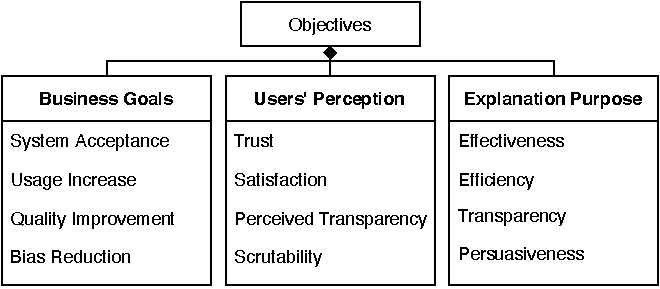
\includegraphics{contents/05_model_description/res/model_objectives_overview.pdf}
    \end{center}
    \caption{Übersicht über die \textit{Objectives} eines erklärbaren Systems}
    \label{fig:model_objectives_overview}
\end{figure}

Wie in \autoref{tab:quality_aspects_of_explanation} zu sehen ist, werden die Qualitätsziele verschieden häufig untersucht. Dies ist ein Indiz dafür, dass die Aspekte einer Struktur bedürfen. Daher schlagen einige Autoren eine hierarchische Anordnung der Qualitätsziele vor \cite{nunes_systematic_2017,tintarev2007survey,waa_evaluating_2021}. Folglich werden die \textit{Objectives} in drei Abstraktionsebenen gegliedert: \textit{Business Goals}, \textit{Users' Perception} und \textit{Explanation Purpose}. Diese Ebenen, die von \citeauthor{nunes_systematic_2017} sowie \citeauthor{tintarev2007survey} vorgeschlagen werden, sind in diesem Modell als konkrete Abstraktionslevel für Qualitätsmodelle (\cite[vgl.][]{schneider2012abenteuer}) zu interpretieren. Die Zuordnung der Qualitätsaspekte zu den Kategorien ist in der \autoref{fig:model_objectives_overview} abgebildet. In \autoref{tab:impact_of_objective_on_explanation} werden die Erwähnungen der drei Zielebenen mit den jeweiligen Synonymen aus der Literatur zusammengefasst.

\begin{table}[htb!]
    \begin{center}
        \begin{tabular}{p{.3\textwidth}p{.41\textwidth}p{.2\textwidth}}
            \hline
            Aspekt    & Synonym & Quellen \\
            \toprule
            Business Goals      & Stakeholder Goals & \cite{nunes_systematic_2017} \\
                                & (Intended) Purpose & \cite{waa_evaluating_2021} \\
                                & Higher-level Goals & \cite{nunes_systematic_2017} \\
                                & Application Level & \cite{sokol_explainability_2020} \\
            \tablerowspacing
            Users' Perception             & User Perceived Quality Factors & \cite{nunes_systematic_2017} \\
                      & (Consumer) Needs & \cite{ehsan_human-centered_2020} \cite{chazette_end-users_nodate} \\
                                & User Goals & \cite{ehsan_human-centered_2020} \\
                                & Intermediate Requirements & \cite{waa_evaluating_2021} \\
                                & Human Level & \cite{sokol_explainability_2020} \\
            \tablerowspacing
            Explanation         & (Explanation) Purpose & \cite{nunes_systematic_2017} \\
            Purpose             & Explanatory Goal & \cite{tintarev_designing_nodate} \cite{balog_measuring_2020} \\
                                & Function Level & \cite{sokol_explainability_2020} \\
            \toprule
        \end{tabular}
    \end{center}
    \caption{Abstraktionsebenen der Zielsetzung bei der Integration von Erklärungen in ein System}
    \label{tab:impact_of_objective_on_explanation}
\end{table}

\paragraph{Business Goals} \textit{Business Goals} sind die Ziele, die für das System im Ganzen gelten. \citeauthor{schneider2012abenteuer} nennt sie im Kontext von Qualitätsmodellen \glqq Allgemeine Qualitätsziele\grqq \cite{schneider2012abenteuer}.

Unter den \textit{Business Goals} werden in der Literatur über die schon genannten Qualitätsaspekte hinaus abstraktere Ziele genannt \cite[vgl. z.~B.][]{cirqueira_scenario-based_2020, nunes_systematic_2017, ribera2019can}. \textit{System Acceptance} beschreibt dabei das Ziel, die Wahrscheinlichkeit zu erhöhen, dass die Entscheidungen eines Systems von \textit{End Usern} akzeptiert werden \cite{cirqueira_scenario-based_2020}. Auch kann ein \textit{Business Goal} sein, die Anzahl der Nutzungen des Systems zu erhöhen. Dies kann sowohl pro Nutzer als auch insgesamt gesehen werden und ist je nach \textit{Context} verschieden definiert \cite{nunes_systematic_2017}. Auch kann ein sehr allgemeines Ziel sein, die grundsätzliche Qualität des Systems zu erhöhen \cite{schneider2012abenteuer}.

\paragraph{User Perception Goals} \textit{User Perception Goals} sind jene Ziele, die direkt durch den \textit{End User} des Systems wahrgenommen werden sollen. Sie tragen zur Erreichung der allgemeinen Ziele auf der höheren Ebene bei. Diese Ziele sind als Zwischenziele hin zu einem konkreten Ziel für zu integrierende Erklärungen zu verstehen.

\paragraph{Explanation Goals} Die \textit{Explanation Goals} sind \glqq konkrete Qualitätsziele\grqq{} für Erklärungen (\cite[vgl.][]{schneider2012abenteuer}). Diese sind allerdings keine konkreten Ziele für eine bestimmte Situation, in der die Erklärungen eingesetzt werden sollen. Hierfür müssen diese bis zu ihrer Messbarkeit weiter verfeinert werden, um daraus Anforderungen zu entwickeln (siehe \autoref{sec:model_evaluation_description}).

\bigskip

Die hier vorgestellten Ziele bei der Integration von Erklärungen stellen keine abgeschlossene oder vollständige Liste dar. Sie dienen im Rahmen des Leitfadens als Überblick über in der Literatur häufig betrachtete Ziele, für deren Erreichung Erklärungen erfolgreich eingesetzt wurden.

\newpage

\smallskip

\noindent\fbox{
    \parbox{0.964\textwidth}{
        \smallskip
        \textbf{RQ1} Welche Rahmenbedingungen haben einen Einfluss auf die Anforderungen für Erklärungen?
        \smallskip
    }
}

\smallskip

Mit dem \textit{Context} des Systems und den \textit{Objectives} für die Integration von Erklärungen wurden im Rahmen des ersten Modellteils die Rahmenbedingungen mit einem direkten Einfluss auf Anforderungen an Erklärungen vorgestellt. Die unter \textit{External Dependencies} zusammengefassten Aspekte und Ausprägungen sind folglich die Antwort auf die erste Forschungsfrage.

Als Hilfsmittel kann der erste Teil des Modells vor allem bei der Anforderungserhebung (\textit{Requirements Elicitation}) und -Analyse (Requirements Analysis) helfen \cite{schneider2012abenteuer}. Auf dieser Basis können Anforderungen formuliert und die Grundlagen für Hypothesen gelegt werden. Folglich wird durch den ersten Modellteil auch die erste Leitfadenanforderung erfüllt ([GR1]).

\smallskip

Im folgenden Abschnitt werden jene Eigenschaften von Erklärungen betrachtet, welche in vorangegangenen Arbeiten bereits zur Umsetzung von Anforderungen verwendet wurden.
